\documentclass{article}
\usepackage{amsfonts, amsmath, amssymb, amsthm} % Math notations imported
\usepackage{enumitem}
\usepackage{graphicx}
\usepackage{setspace}
\usepackage{indentfirst}
\usepackage[margin=1in]{geometry}
\graphicspath{{./images/}} % Path to images

% \begin{figure}[htb!]
%      \centering
%      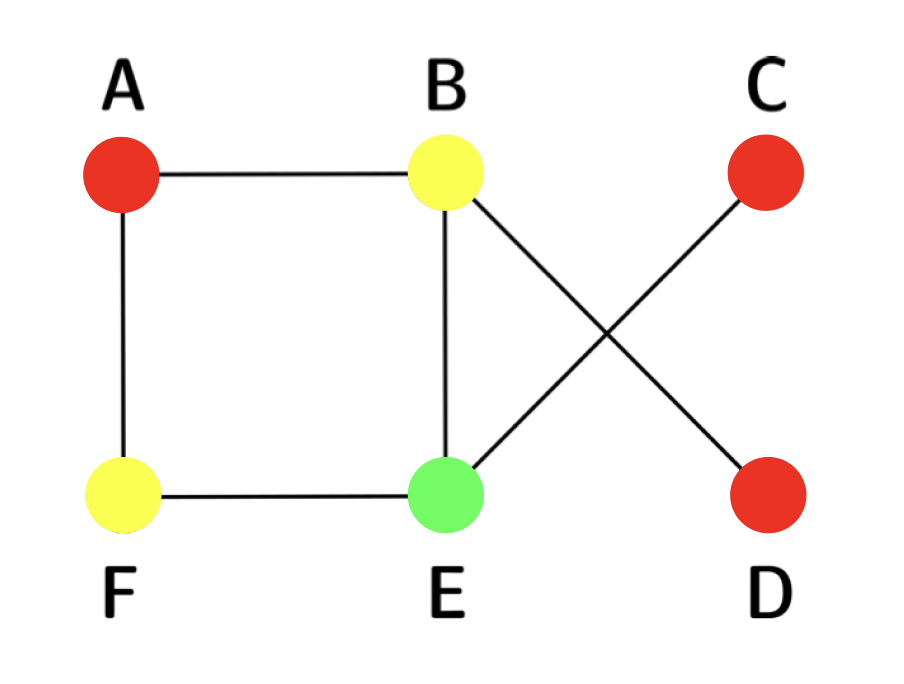
\includegraphics[scale=0.5]{coloring.png}
%      \caption{Coloring of the graph.}
% \end{figure}

\newtheorem{thm}{Theorem}
\newtheorem{proposition}[thm]{Proposition}
\newtheorem{cor}[thm]{Corollary}

% title information
\title{Math 104 HW2}
\author{Neo Lee}
\date{09/08/2023}

\setstretch{1.15}
% main content
\begin{document} 

% placing title information; comment out if using fancyhdr
\maketitle 

\section*{Exercise 4.1}
For each set below that is bounded above, list three upper bounds for the set. Otherwise write 
"NOT BOUNDED ABOVE". 

\textbf{(a)} [0,1]
\begin{proof}[Solution]
    \{2, 3, 4\}
\end{proof}

\textbf{(c)} \{2,7\}
\begin{proof}[Solution]
    \{8, 9, 10\}
\end{proof}

\textbf{(e)} $\{\frac{1}{n}:n\in\mathbb{N}\}$
\begin{proof}[Solution]
    \{8, 9, 10\}
\end{proof}

\textbf{(g)} [0,1] $\cup$ [2,3]
\begin{proof}[Solution]
    \{8, 9, 10\}
\end{proof}

\textbf{(i)} $\cap^\infty_{n=1}\left[\frac{-1}{n}, 1+\frac{1}{n}\right]$
\begin{proof}[Solution]
    \{8,9,10\}
\end{proof}

\textbf{(k)} $\{n+\frac{(-1)^n}{n}:n\in\mathbb{N}\}$
\begin{proof}[Solution]
    NOT BOUNDED ABOVE
\end{proof}

\textbf{(m)} $\{r\in\mathbb{Q}:r^2<4\}$
\begin{proof}[Solution]
    \{8,9,10\}
\end{proof}

\textbf{(o)} $\{x\in\mathbb{R}:x<0\}$
\begin{proof}[Solution]
    \{8,9,10\}
\end{proof}

\textbf{(q)} \{0, 1, 2, 4, 8, 16\}
\begin{proof}[Solution]
    \{20, 30, 40\}
\end{proof}

\textbf{(s)} $\{\frac{1}{n}:n\in\mathbb{N} \emph{ and } n \emph{ is prime}\}$
\begin{proof}[Solution]
    \{20, 30, 40\}
\end{proof}

\textbf{(u)} $\{x^2:x\in\mathbb{R}\}$
\begin{proof}[Solution]
    NOT BOUNDED ABOVE
\end{proof}

\textbf{(w)} $\{sin\left(\frac{n\pi}{3}\right):n\in\mathbb{N}\}$
\begin{proof}[Solution]
    \{20, 30, 40\}
\end{proof}


\section*{Exercise 4.2}
Repeat Exercise 4.1 for lower bounds.

\textbf{(a)} [0,1]
\begin{proof}[Solution]
    \{-2, -3, -4\}
\end{proof}

\textbf{(c)} \{2,7\}
\begin{proof}[Solution]
    \{-8, -9, -10\}
\end{proof}

\textbf{(e)} $\{\frac{1}{n}:n\in\mathbb{N}\}$
\begin{proof}[Solution]
    \{-8, -9, -10\}
\end{proof}

\textbf{(g)} [0,1] $\cup$ [2,3]
\begin{proof}[Solution]
    \{-8, -9, -10\}
\end{proof}

\textbf{(i)} $\cap^\infty_{n=1}\left[\frac{-1}{n}, 1+\frac{1}{n}\right]$
\begin{proof}[Solution]
    \{-8,-9,-10\}
\end{proof}

\textbf{(k)} $\{n+\frac{(-1)^n}{n}:n\in\mathbb{N}\}$
\begin{proof}[Solution]
    \{-8,-9,-10\}
\end{proof}

\textbf{(m)} $\{r\in\mathbb{Q}:r^2<4\}$
\begin{proof}[Solution]
    \{-8,-9,-10\}
\end{proof}

\textbf{(o)} $\{x\in\mathbb{R}:x<0\}$
\begin{proof}[Solution]
    NOT BOUNDED BELOW
\end{proof}

\textbf{(q)} \{0, 1, 2, 4, 8, 16\}
\begin{proof}[Solution]
    \{-20, -30, -40\}
\end{proof}

\textbf{(s)} $\{\frac{1}{n}:n\in\mathbb{N} \emph{ and } n \emph{ is prime}\}$
\begin{proof}[Solution]
    \{-20, -30, -40\}
\end{proof}

\textbf{(u)} $\{x^2:x\in\mathbb{R}\}$
\begin{proof}[Solution]
    \{-20, -30, -40\}
\end{proof}

\textbf{(w)} $\{sin\left(\frac{n\pi}{3}\right):n\in\mathbb{N}\}$
\begin{proof}[Solution]
    \{-20, -30, -40\}
\end{proof}

\section*{Exercise 4.8}
Let $S$ and $T$ be nonempty subsets of R with the following property: $s\le t$ for all $s\in S$ and 
$t\in T$.
\begin{enumerate}[label=(\alph*)]
    \item Oberserve that $S$ is bounded above and $T$ is bounded below. 
    \begin{proof}
        $T\subseteq U(S), S\subseteq L(T)$.
    \end{proof}
    \item \begin{proposition}
        Sup $S\le$ inf $T$.
    \end{proposition}
    \begin{proof}
        Assume for the sake of contradiction that sup $S >$ inf $T$. Then inf $T$ can be written as 
        inf $T$ = sup $S - \epsilon$ for some $\epsilon > 0$. Notice that there exists $s\in S$ 
        such that $s >$ sup $S - \epsilon$ [otherwise sup$S -\epsilon$ would be a 
        smaller upper bound]. This implies that there exists $s\in S$ such that $s > $ inf $T$. That 
        means inf $T$ is not the largest lower bound of $T$ [$s$ is a larger lower bound], which is 
        a contradiction. Hence, sup $S\le$ inf $T$.
    \end{proof}
    \item Give an exampe of such sets $S$ and $T$ where $S\cap T$ is nonempty.
    \begin{proof}[Solution]
        $S = \{s \le 0 :s \in\mathbb{R}\}$, $T = \{t \ge 0 :t \in\mathbb{R}\}$, $S\cap T = \{0\}$.
    \end{proof}
    \item Give an example of sets $S$ and $T$ where sup $S=$ inf $T$ and $S\cap T$ is an empty set.
    \begin{proof}[Solution]
        $S = \{s < 0 :s \in\mathbb{R}\}$, $T = \{t > 0 :t \in\mathbb{R}\}$, $S\cap T = \emptyset$.
    \end{proof}
\end{enumerate}

\section*{Exercise 4.14}
Let $A$ and $B$ be nonempty bounded subsets of $\mathbb{R}$, and let $A + B$ be the set of all 
sums $a+b$ where $a\in A$ and $b\in B$.
\begin{enumerate}[label=(\alph*)]
    \item \begin{proposition}
        Sup $(A+B) = $ sup $A$ + sup $B$. Hint: To show sup $A$ + sup $B\le$ sup $(A+B)$, show that 
        for each $b \in B$, sup $(A+B)-b$ is an upper bound for $A$, hence sup $A \le$ sup 
        $(A + B) - b$. Then show sup $(A + B)$ - sup $A$ is an upper bound for $B$.
    \end{proposition}
    \begin{proof}
        We proceed by first showing $\emph{sup}(A+B)\le\emph{sup}A+\emph{sup}B$, then showing   
        $\emph{sup}(A+B)\ge\emph{sup}A+\emph{sup}B$.

        \underline{$\emph{sup}(A+B)\le\emph{sup}A+\emph{sup}B$}. For all $x\in A+B$, $x = a
        + b$ for $a\in A, b\in B$. Hence, $x = a + b \le \emph{sup}A+\emph{sup}B \Rightarrow 
        \emph{sup}A+\emph{sup}B\subseteq U(A+B)\Rightarrow \emph{sup}(A+B)\le \emph{sup}A+
        \emph{sup}B$.

        \underline{$\emph{sup}(A+B)\ge\emph{sup}A+\emph{sup}B$}. Assume for the sake of 
        contradiction that $\emph{sup}(A+B)<\emph{sup}A+\emph{sup}B$. Then $\emph{sup}(A+B) = 
        \emph{sup}A+\emph{sup}B-\epsilon$ for some $\epsilon > 0$. Notice $\exists b\in B$ and 
        $\exists a\in A$ such that $\emph{sup}A - \epsilon/2 < a$ and $\emph{sup}B - \epsilon/2 < 
        b$. Then $\emph{sup}A + \emph{sup}B - \epsilon =\emph{sup}(A+B)< a + b$, which is a 
        contradiction. Hence, $\emph{sup}(A+B)\ge\emph{sup}A+\emph{sup}B$.
    \end{proof}
    \item \begin{proposition}
        Inf $(A+B) = $ inf $A$ + inf $B$.
    \end{proposition}
    \begin{proof}
        We proceed by first showing $\emph{inf}(A+B)\ge\emph{inf}A+\emph{inf}B$, then showing   
        $\emph{inf}(A+B)\le\emph{inf}A+\emph{inf}B$.

        \underline{$\emph{inf}(A+B)\ge\emph{inf}A+\emph{inf}B$}. For all $x\in A+B$, $x = a
        + b$ for $a\in A, b\in B$. Hence, $x = a + b \ge \emph{inf}A+\emph{inf}B \Rightarrow 
        \emph{inf}A+\emph{inf}B\subseteq L(A+B)\Rightarrow \emph{inf}(A+B)\ge \emph{inf}A+
        \emph{inf}B$.

        \underline{$\emph{inf}(A+B)\le\emph{inf}A+\emph{inf}B$}. Assume for the sake of 
        contradiction that $\emph{inf}(A+B)>\emph{inf}A+\emph{inf}B$. Then $\emph{inf}(A+B) = 
        \emph{inf}A+\emph{inf}B+\epsilon$ for some $\epsilon > 0$. Notice $\exists b\in B$ and 
        $\exists a\in A$ such that $\emph{inf}A + \epsilon/2 > a$ and $\emph{inf}B + \epsilon/2 > 
        b$. Then $\emph{inf}A + \emph{inf}B + \epsilon =\emph{inf}(A+B)> a + b$, which is a 
        contradiction. Hence, $\emph{inf}(A+B)\le\emph{inf}A+\emph{inf}B$.
    \end{proof}
\end{enumerate}

\section*{Exercise 4.16}
\begin{proposition}
    Sup $\{r\in\mathbb{Q}:r<a\} = a$ for each $a\in\mathbb{R}$.
\end{proposition}
\begin{proof}
    Denote $A = \{r\in\mathbb{Q}:r<a\}$. We proceed by first showing $a$ is an upper bound of $A$, 
    then showing $a$ is the least upper bound of $A$.

    \underline{$a$ is an upper bound of $A$}. For all $r\in A$, $r < a \Rightarrow r\le a$. Hence, 
    $a$ is an upper bound of $A$. Trivial.

    \underline{$a$ is the least upper bound of $A$}. Assume for the sake of contradiction that 
    $\emph{sup}A < a$, then $\emph{sup}A = a - \epsilon$ for some $\epsilon > 0$. Now by the 
    Archimedean Property, there exists $n\in\mathbb{N}$ such that $1/n < \epsilon$. Then, we can 
    take $r = \emph{sup}A + 1/n = a - \epsilon + 1/n < a$. This implies that $r\in A$ and $r > 
    \emph{sup}A$, which is a contradiction. Hence, $a$ is the least upper bound of $A$.
\end{proof}

\section*{Exercise 5.5}
\begin{proposition}
    Inf $S \le$ sup $S$ for every nonempty subset of $\mathbb{R}$. Consider both bounded and 
    unbounded sets.
\end{proposition}
\begin{proof} 
    \indent
    \begin{enumerate}[label = Case \arabic*:]
        \item $S$ is bounded above and below. Then $\emph{inf}S \le s \in S$ 
        and $\emph{sup}S \ge s \in S$ for $\emph{inf}S, \emph{sup}S \in \mathbb{R}$. 
        Hence, $\emph{inf}S \le s\le \emph{sup}S$.

        \item $S$ is bounded above and unbounded below. Then $\emph{inf}S = -\infty\le s \in S$ and 
        $\emph{sup}S \in\mathbb{R} \ge s\in S$. Obviously, $-\infty \le \emph{sup}S$.

        \item $S$ is unbounded above and bounded below. Then $\emph{inf}S \in\mathbb{R}\le s \in S$ 
        and $\emph{sup}S = \infty \ge s\in S$. Obviously, $\emph{inf}S \le \infty$.

        \item $S$ is unbounded above and below. Then $\emph{inf}S = -\infty$ and $\emph{sup}S = 
        \infty$. Obviously, $-\infty \le \infty$.
    \end{enumerate}
\end{proof}

\end{document}
